\section{Additional competitive-to-monopoly simulation results}
\label{app:rewrite-competitive-transition}

I supplement the $\sigma=1.5$ comparison in
Section~\ref{subsec:rewrite-competitive-transition} with the original
four-elasticity exercises at both research productivities. No additional
equilibria are computed for this presentation. The level figures retain
the three windows used in that section; the growth, price, and
distributional figures below show
two pre-event years and years 0--10 above, with years 10--500 below.
Thin horizontal lines show continued competition; black dotted
long-run lines show the analytical monopoly limits at $\sigma=1.5$.
The benchmark lines also distinguish the
competitive income shares from the monopoly limits: competitive
AI revenue pays for inference, whereas monopoly revenue also
finances research and developer profit.
The date-zero level changes are not finite growth rates: open and
filled dots distinguish the values on either side of the event, and
growth curves describe the smooth trajectory on each side separately.

\begin{table}[H]
 \centering
 \caption{Competitive initial capital and the impact of exclusive AI rights}
 \label{tab:rewrite-competitive-transition}
 \small\setstretch{1.0}
 \begin{tabular}{cccc}
 \toprule
 $\sigma$ & $K_0$ & Change in output & Change in wage\\
 \midrule
 0.9 & 6.235 & $-32.4\%$ & $-36.6\%$\\
 1.0 & 6.278 & $-17.6\%$ & $-17.6\%$\\
 1.1 & 6.324 & $-13.7\%$ & $-11.9\%$\\
 1.5 & 6.535 & $-10.4\%$ & $-5.4\%$\\
 \bottomrule
 \end{tabular}
 \par\vspace{4pt}
 \parbox{0.95\textwidth}{\footnotesize\emph{Notes:} The capital stocks are
 derived from the competitive BGP, not selected independently. All other
 parameters and initial stocks are in Table~\ref{tab:rewrite-rsi-parameters}.
 Changes compare levels immediately after and before the grant. They are
 identical for both values of $\chi$, since $K$ and $B$ cannot jump.
 The ratio $K_0/Y_{0^-}=3.3$ applies before the grant, not after output falls.}
\end{table}

\paragraph{Level comparisons across elasticities.}
Figures~\ref{fig:rewrite-competitive-high-levels}
and~\ref{fig:rewrite-competitive-low-levels} preserve the level comparisons
for all four elasticities. Research can produce level gains even where it
does not permanently raise growth. With $\chi=7.5$, output first regains
its competitive counterpart around year 18.2 at $\sigma=1.1$ and year 46.9
at $\sigma=1$. With $\chi=1.5$, those recoveries occur around years 87.3
and 212.3. At $\sigma=0.9$, neither output nor wages regain their
competitive counterparts within 500 years under either $\chi$.
The initial AI-service price in that case is about 131 times its competitive
level, a large distortion implied by the illustrative parameters rather
than an empirical estimate. These recovery dates compare contemporaneous
levels; they do not rank welfare.

\begin{figure}[H]
 \centering
 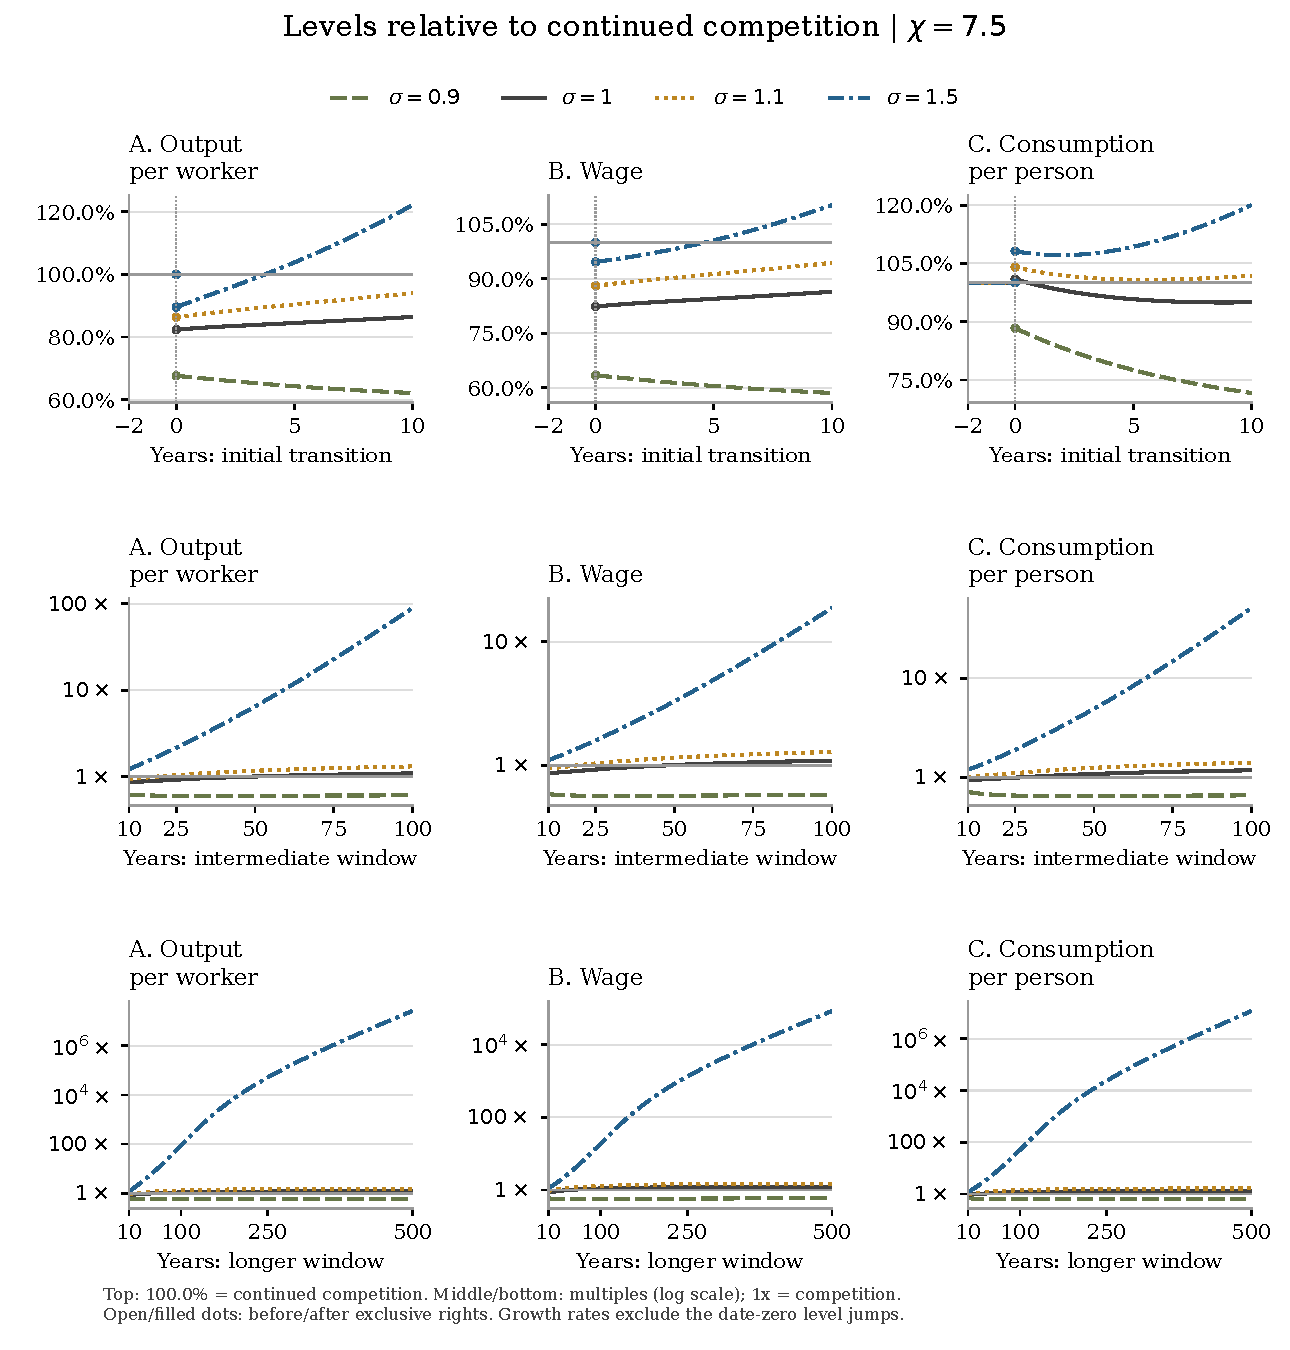
\includegraphics[width=\textwidth]{figures_rewrite/competitive_to_monopoly/competitive_to_monopoly_chi_7_5_levels.pdf}
 \caption{From competition to monopoly with RSI, $\chi=7.5$: levels
 relative to continued competition for all four elasticities. The rows
 cover years $-2$--10, 10--100, and 10--500. The upper row uses percentages;
 the middle and lower rows use multiples on logarithmic scales.
 The horizontal benchmark is $100.0\%$ or $1\times$. Open and filled dots
 mark levels before and after the grant. Vertical scales differ across
 windows and between the two research-productivity exercises.}
 \label{fig:rewrite-competitive-high-levels}
\end{figure}

\begin{figure}[H]
 \centering
 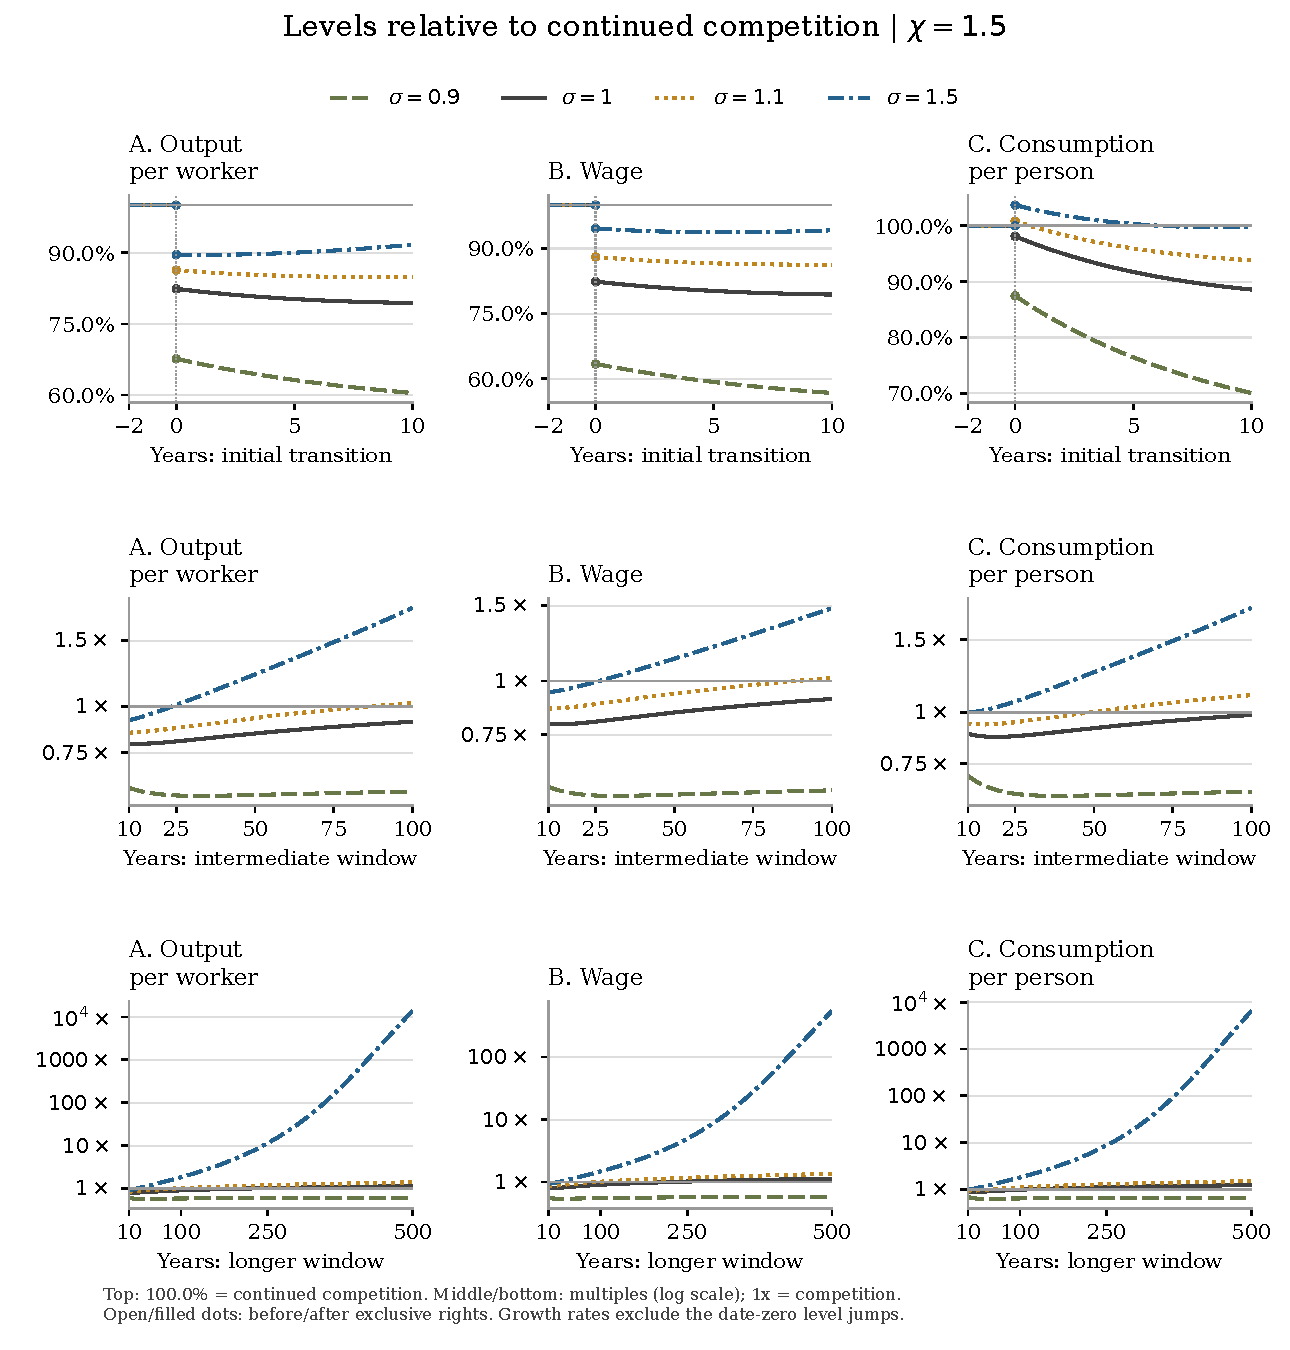
\includegraphics[width=\textwidth]{figures_rewrite/competitive_to_monopoly/competitive_to_monopoly_chi_1_5_levels.pdf}
 \caption{From competition to monopoly with RSI, $\chi=1.5$: output
 per worker, wages, and consumption per person relative to continued
 competition for all four elasticities. Windows, normalizations, and
 line styles match Figure~\ref{fig:rewrite-competitive-high-levels}.
 Vertical scales are fitted to this exercise.}
 \label{fig:rewrite-competitive-low-levels}
\end{figure}

\paragraph{Initial conditions and numerical checks.}
I obtain each competitive initial stock by imposing $r=\rho+\gamma$
with the marginal-cost pricing condition $p_X=1/B_0$. Pre-event
consumption follows from the resource constraint with $M=0$ and
$\dot K=(n+\gamma)K$. The post-event calculation uses the same monopoly
BVP and equilibrium checks as Appendix~\ref{app:rewrite-algorithm}.
Previously computed RSI-activation trajectories supply numerical
initial guesses, but I solve again at the competitive $K_0$, imposing
neither their consumption nor their research choices. All eight
paths pass the same residual, horizon-refinement, transversality,
and developer-optimality checks; no tolerance is relaxed.

\paragraph{Higher research productivity.}
Figures~\ref{fig:rewrite-competitive-high-growth}--\ref{fig:rewrite-competitive-high-distribution}
report $\chi=7.5$. Unlike the pure RSI-activation experiment, the grant
immediately reduces the return on capital: output falls while capital
cannot jump, so equation~\eqref{eq:rewrite-capital-return} implies a
lower interest rate. The Euler equation~\eqref{eq:rewrite-euler}
then gives lower consumption growth immediately after the grant,
even where the level of consumption jumps upward. Subsequent RSI
and capital adjustment determine recovery. Research absorbs resources
before its gains are fully realized, and the distribution panels
separate developer net profit from expenditure on inference and research.

\begin{figure}[H]
 \centering
 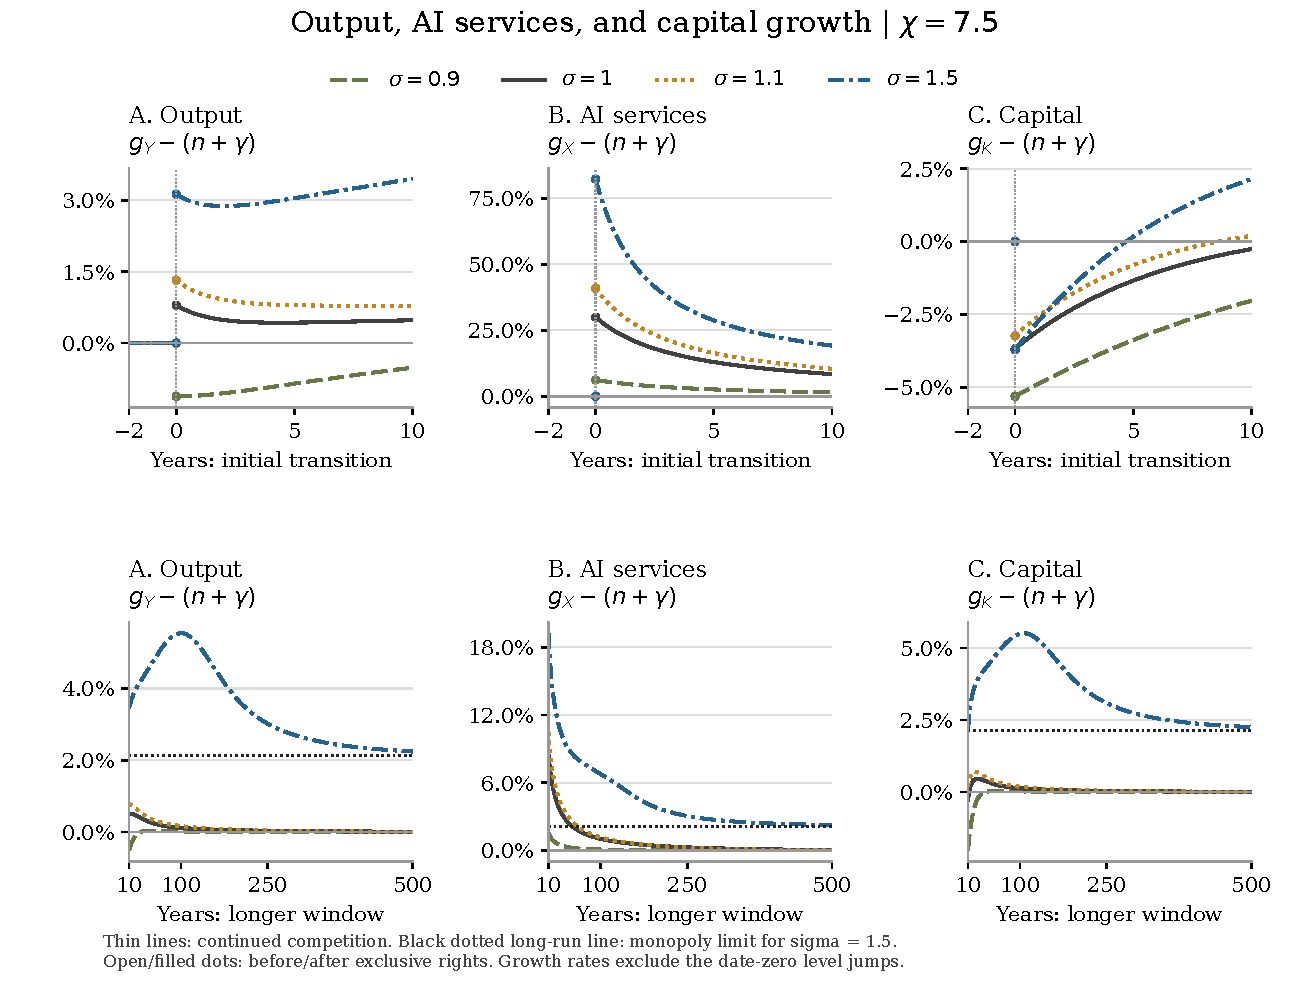
\includegraphics[width=\textwidth]{figures_rewrite/competitive_to_monopoly/competitive_to_monopoly_chi_7_5_accumulation_growth.pdf}
 \caption{Competition to monopoly, $\chi=7.5$: annual growth of output,
 AI services, and capital relative to effective labor. Zero denotes
 growth at $n+\gamma$. Growth rates exclude the discrete level changes
 at date zero.}
 \label{fig:rewrite-competitive-high-growth}
\end{figure}

\begin{figure}[H]
 \centering
 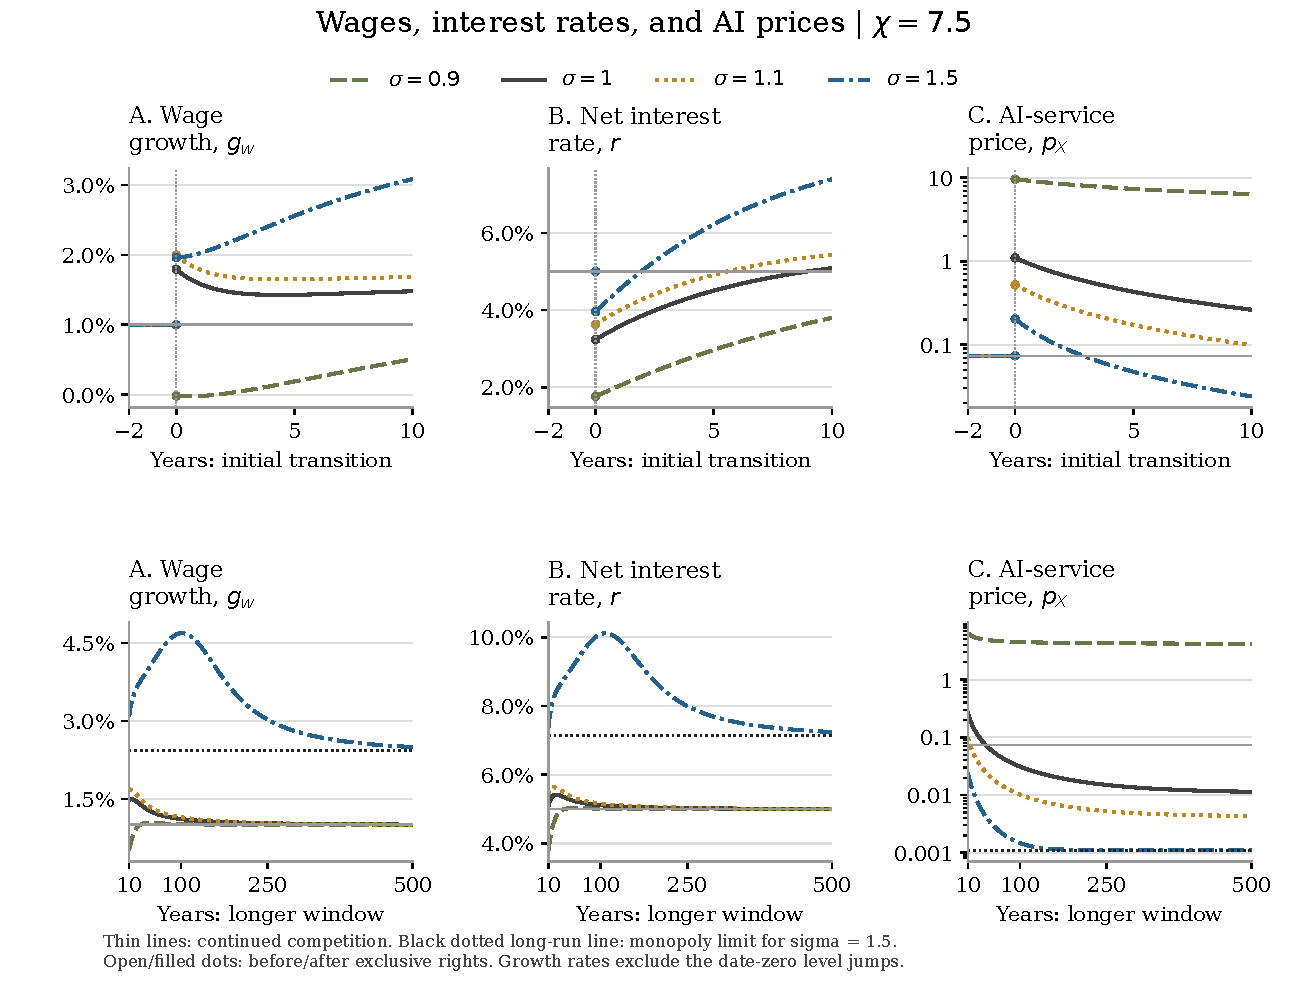
\includegraphics[width=\textwidth]{figures_rewrite/competitive_to_monopoly/competitive_to_monopoly_chi_7_5_growth_returns.pdf}
 \caption{Competition to monopoly, $\chi=7.5$: annual wage growth,
 net interest, and AI-service prices. Prices are measured in final-good
 units on a logarithmic scale. The wage level falls at the grant;
 panel A reports wage growth on either side, not that level change.}
 \label{fig:rewrite-competitive-high-prices}
\end{figure}

\begin{figure}[H]
 \centering
 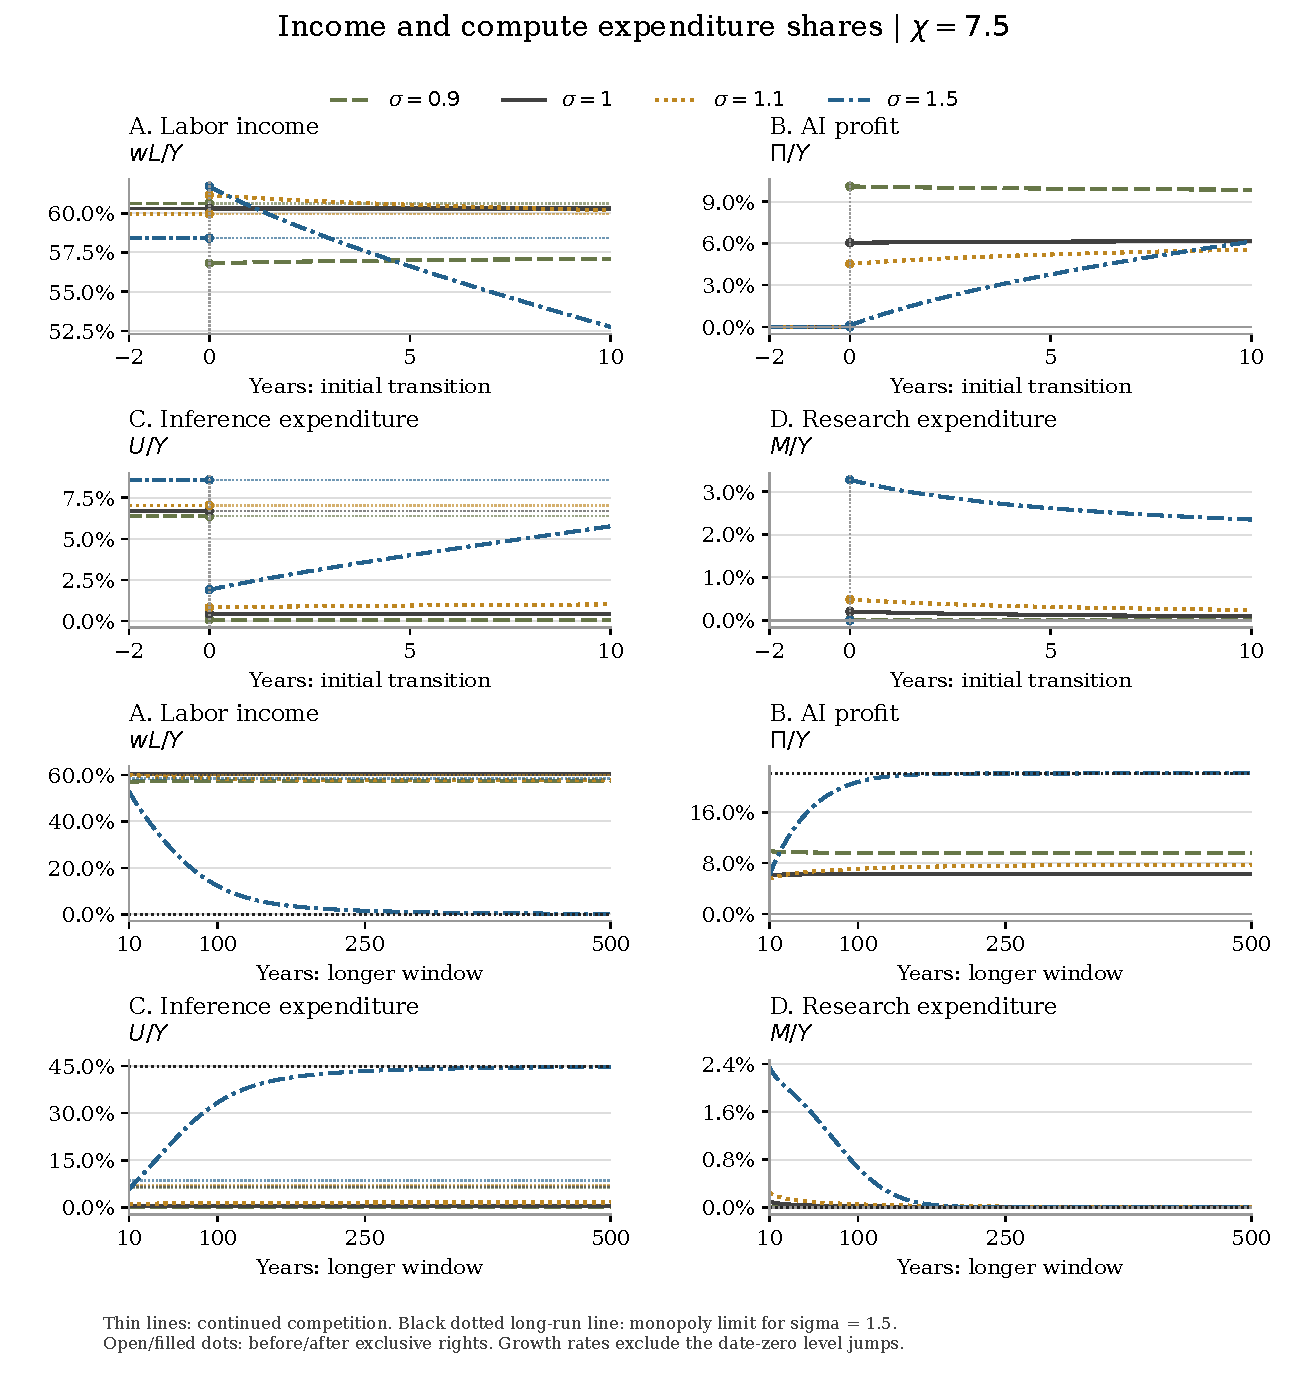
\includegraphics[width=\textwidth]{figures_rewrite/competitive_to_monopoly/competitive_to_monopoly_chi_7_5_distribution.pdf}
 \caption{Competition to monopoly, $\chi=7.5$: labor income, developer
 net profit, inference expenditure, and research expenditure as shares
 of output. The first two rows cover years $-2$--10; the last two
 cover years 10--500. Gross capital income remains $33.0\%$ of output.}
 \label{fig:rewrite-competitive-high-distribution}
\end{figure}

\paragraph{Lower research productivity.}
Figures~\ref{fig:rewrite-competitive-low-growth}--\ref{fig:rewrite-competitive-low-distribution}
report $\chi=1.5$. The impact pricing distortion is unchanged, but
the initial research allocation and efficiency growth are smaller.
At $\sigma=1.5$, the eventual rise in growth and decline in labor's
share emerge later. At year 500, growth and returns still exceed
their monopoly limits, so the final displayed values should not be
read as those limits.

\begin{figure}[H]
 \centering
 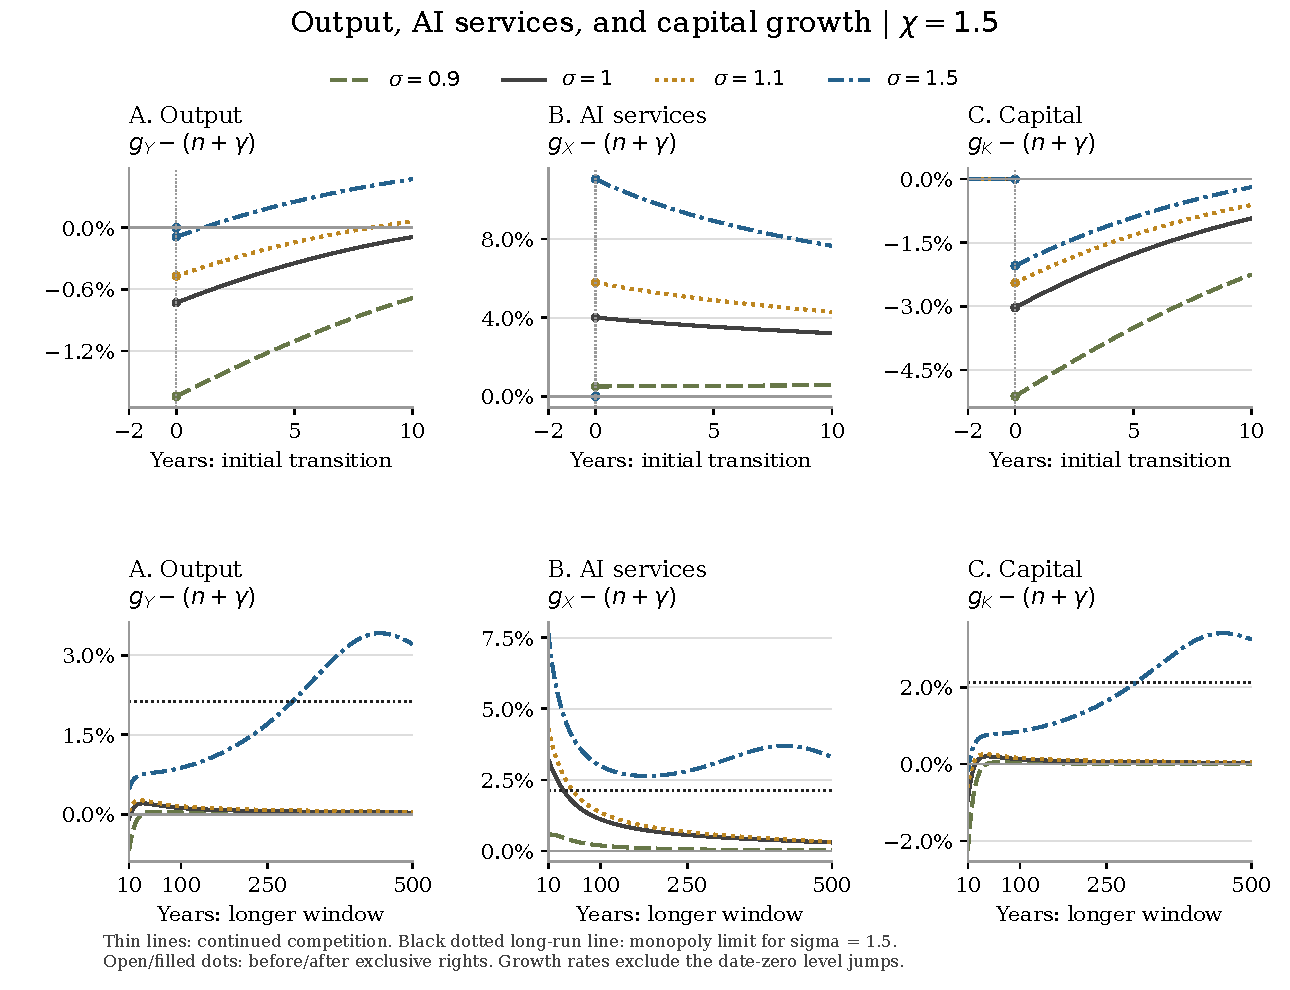
\includegraphics[width=\textwidth]{figures_rewrite/competitive_to_monopoly/competitive_to_monopoly_chi_1_5_accumulation_growth.pdf}
 \caption{Competition to monopoly, $\chi=1.5$: annual growth of output,
 AI services, and capital relative to effective labor. Windows and
 benchmarks match Figure~\ref{fig:rewrite-competitive-high-growth}.}
 \label{fig:rewrite-competitive-low-growth}
\end{figure}

\begin{figure}[H]
 \centering
 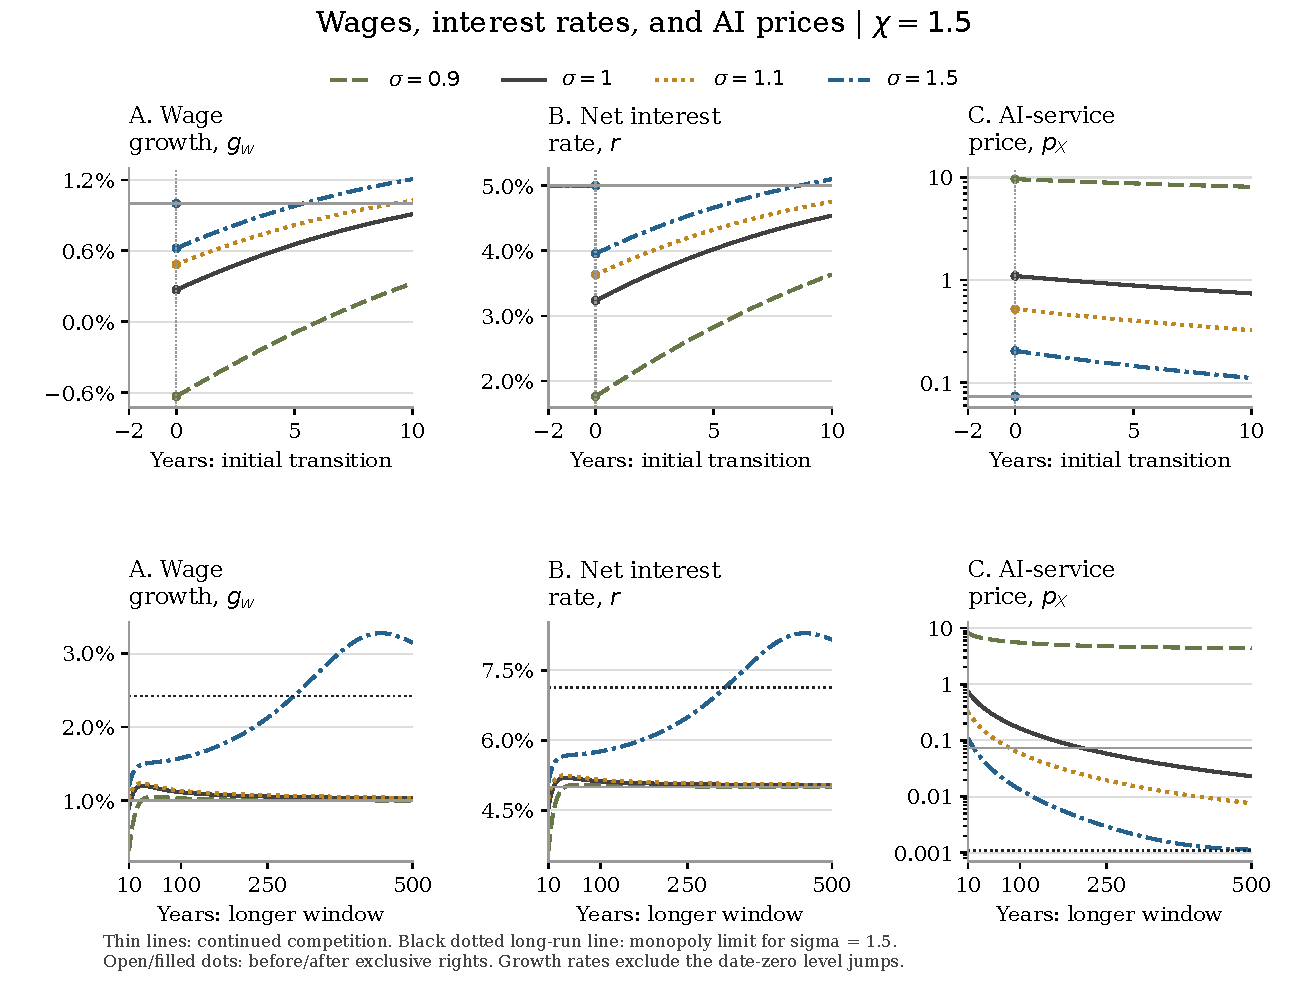
\includegraphics[width=\textwidth]{figures_rewrite/competitive_to_monopoly/competitive_to_monopoly_chi_1_5_growth_returns.pdf}
 \caption{Competition to monopoly, $\chi=1.5$: annual wage growth,
 net interest, and AI-service prices in final-good units. Windows,
 benchmarks, and the logarithmic price scale match
 Figure~\ref{fig:rewrite-competitive-high-prices}.}
 \label{fig:rewrite-competitive-low-prices}
\end{figure}

\begin{figure}[H]
 \centering
 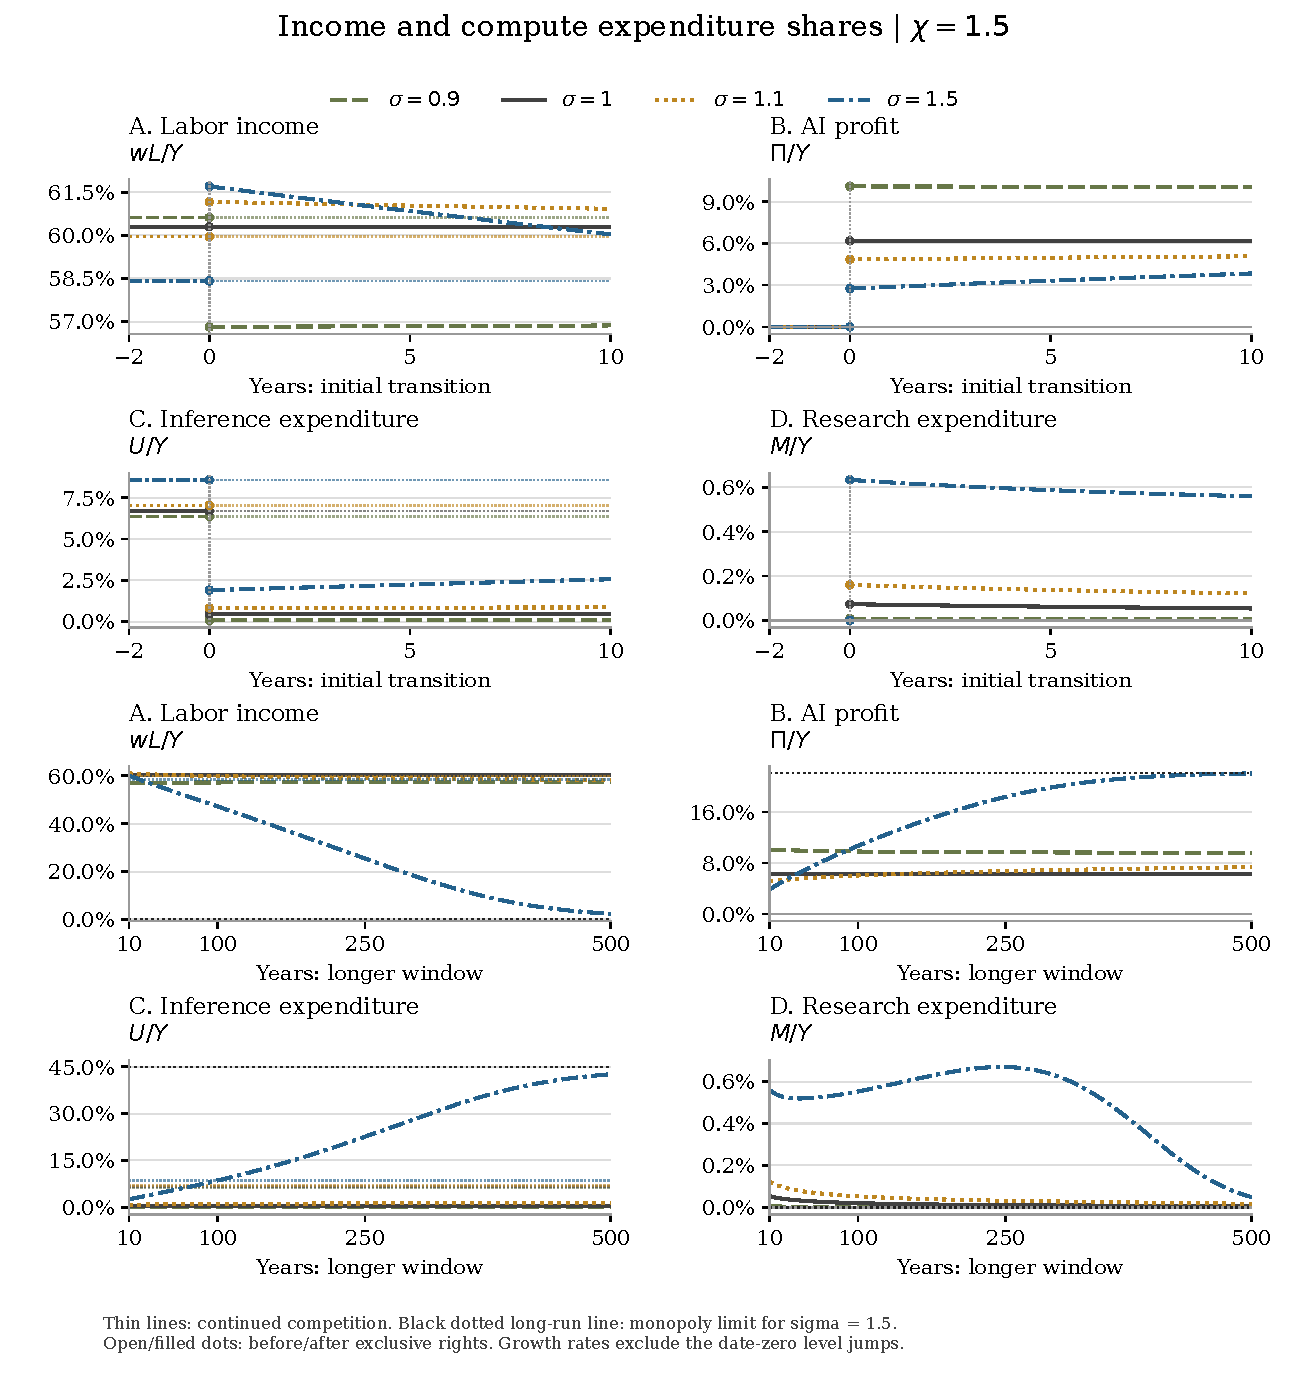
\includegraphics[width=\textwidth]{figures_rewrite/competitive_to_monopoly/competitive_to_monopoly_chi_1_5_distribution.pdf}
 \caption{Competition to monopoly, $\chi=1.5$: labor income, developer
 net profit, inference expenditure, and research expenditure relative
 to output. Layout and benchmarks match
 Figure~\ref{fig:rewrite-competitive-high-distribution}.}
 \label{fig:rewrite-competitive-low-distribution}
\end{figure}

\paragraph{Replication.}
The repository's
\href{https://github.com/oliverpardo1979/ai-growth-and-labor/blob/main/COMPETITIVE_TRANSITION.md}
{competitive-transition guide} records the parameters, the institutional
experiment, and the replication commands. The driver is
\path{scripts/simulate_competitive_to_monopoly.py}; the renderer is
\path{scripts/report_competitive_to_monopoly.py}.
The guide links to the separate results folders for each research
productivity, containing the original paths, competitive benchmarks,
impact changes, and numerical audits.
The main-text $\sigma=1.5$ comparison is rendered by
\path{scripts/report_competitive_main_comparison.py}, which reads these
same audited paths without changing them.
Figure windows only select dates from those stored paths; they do not
change the simulated economy or the numerical solution horizon.

The repository's
\href{https://github.com/oliverpardo1979/ai-growth-and-labor/blob/main/MONOPOLY_GROWTH_REVERSAL.md}
{growth-reversal replication guide} records the separate input choices,
data, audit reports, and commands. The original growth-reversal
experiment, initialized at $A_0=N_0=1$, remains archived in separate
files; the other simulation exercises are unchanged.

\paragraph{Growth reversal under exclusive rights.}
For Section~\ref{subsec:rewrite-monopoly-growth-reversal}, I first
construct a competitive prehistory with $B=B_0$ above the competitive
threshold. At the start of this prehistory, I normalize $A=N=1$ and
set $K=14{,}047.3$, the limiting monopoly capital--effective-labor ratio
at the chosen upper bound. These seed values are illustrative; they
are not the stocks at the monopoly grant. I advance the competitive
path to year 190, the first whole year at which the three rates in
\eqref{eq:rewrite-competitive-ai-growth} are each within 0.1 percentage
point of their limits; all subsequent annual observations through
year 1,000 also satisfy this criterion. I then set that date to zero
and inherit $A$, $N$, and $K$ without changing units. Re-solving the
competitive equilibrium from those stocks reproduces the continued
prehistory path to within $10^{-9}$ in log levels over the next 500
years. The figures include its last ten pre-grant years.

I solve the competitive
resource constraint and Euler equation in
\eqref{eq:rewrite-competitive-normalized}, with $M=0$ and $B=B_0$,
using the inherited capital stock and the terminal condition
$C/K\to\rho-n$ from
\eqref{eq:rewrite-competitive-capital-growth}.
The numerical coordinates are $\log(C/K)$ and
$\log(K/(AL))-[\mathcal R^{\mathrm{mc}}(B_0)-\rho-\gamma]t$.
Removing the limiting trend avoids extremely large levels without
imposing balanced growth on the transition. I use the same
\texttt{scipy.integrate.solve\_bvp} routine described in the numerical
appendix. Extending its horizon from 1,200 to 1,800 years changes
these coordinates by less than $10^{-9}$ over the displayed 500 years;
independent finite-difference residuals are below $10^{-9}$.
The static supply condition, positive allocation, limiting growth
rates, and household transversality diagnostics also pass the checks.

I solve the two monopoly paths using the existing continuation method,
without changing its equilibrium-admission tolerances. Their final
solution horizon is about 4,592 years, although the figures display
only the first 500 years. Both pass the equation, horizon-extension,
transversality, and developer-optimality checks, including denser
checks over the first decade.
